\documentclass[tikz,border=8pt]{standalone}
\usepackage{tikz}
\usepackage{amsmath}
\usetikzlibrary{arrows.meta, positioning, calc}

% ── Colour palette ─────────────────────────────────────────────────────────
\definecolor{cCtrl} {RGB}{255,243,215}   % amber  – user / control nodes
\definecolor{cCtrlB}{RGB}{175,115,35}
\definecolor{cMdl}  {RGB}{218,233,252}   % sky    – learned / model nodes
\definecolor{cMdlB} {RGB}{35,98,172}
\definecolor{cFilm} {RGB}{238,222,255}   % violet – FiLM conditioning
\definecolor{cFilmB}{RGB}{115,52,155}
\definecolor{cOut}  {RGB}{218,245,225}   % mint   – outputs
\definecolor{cOutB} {RGB}{50,125,70}
\definecolor{cGray} {RGB}{243,245,248}
\definecolor{cDark} {RGB}{32,42,52}

\begin{document}
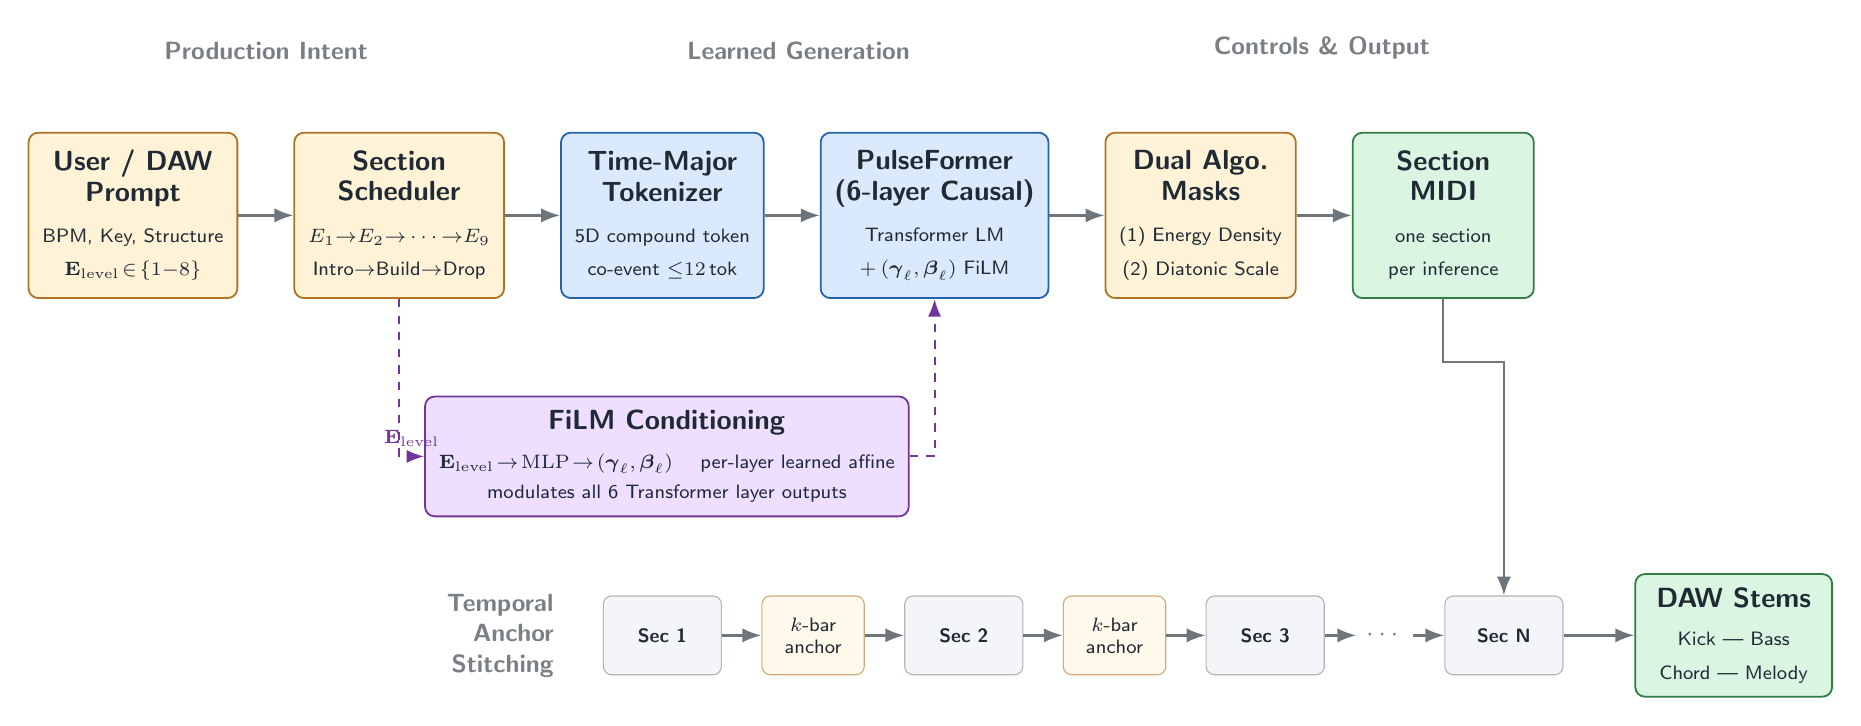
\begin{tikzpicture}[
  font=\sffamily,
  >=Latex,
  % ── shared box style
  pipe/.style={
    draw, rounded corners=3.5pt, align=center,
    inner sep=5pt, text=cDark, line width=0.65pt,
    minimum width=23mm, minimum height=21mm
  },
  ctrl/.style ={pipe, fill=cCtrl,  draw=cCtrlB},
  mdl/.style  ={pipe, fill=cMdl,   draw=cMdlB},
  outp/.style ={pipe, fill=cOut,   draw=cOutB},
  % ── FiLM bypass box (wider, shorter)
  filmst/.style={
    draw=cFilmB, fill=cFilm,
    rounded corners=3.5pt, align=center,
    inner sep=5pt, text=cDark, line width=0.65pt,
    minimum width=44mm, minimum height=14mm
  },
  % ── stitching row boxes
  sml/.style={
    draw=cDark!35, fill=cGray,
    rounded corners=3pt, align=center,
    inner sep=3pt, font=\scriptsize\sffamily, text=cDark,
    minimum width=15mm, minimum height=10mm
  },
  anc/.style={sml, fill=cCtrl!50, draw=cCtrlB!60, minimum width=13mm},
  % ── arrows
  arr/.style ={->, draw=cDark!65,  line width=0.85pt},
  darr/.style={->, draw=cFilmB,    line width=0.75pt, dashed},
  % ── labels
  phlbl/.style={font=\small\sffamily\bfseries, text=cDark!60, align=center},
]

%% ═══════════════════════════════════════════════════════════════════════════
%%  ROW 1 — Main Pipeline  (6 boxes, 23 mm wide, 7 mm gaps)
%% ═══════════════════════════════════════════════════════════════════════════

\node[ctrl] (A) at (0,0) {
  \textbf{User / DAW}\\[-1pt]\textbf{Prompt}\\[3pt]
  \scriptsize BPM,\ Key,\ Structure\\
  \scriptsize $\mathbf{E}_{\mathrm{level}}\!\in\!\{1{-}8\}$
};

\node[ctrl, right=7mm of A] (B) {
  \textbf{Section}\\[-1pt]\textbf{Scheduler}\\[3pt]
  \scriptsize $E_1{\to}E_2{\to}\cdots{\to}E_9$\\
  \scriptsize Intro$\to$Build$\to$Drop
};

\node[mdl, right=7mm of B] (C) {
  \textbf{Time-Major}\\[-1pt]\textbf{Tokenizer}\\[3pt]
  \scriptsize 5D compound token\\
  \scriptsize co-event ${\leq}12$\,tok
};

\node[mdl, right=7mm of C] (D) {
  \textbf{PulseFormer}\\[-1pt]\textbf{(6-layer Causal)}\\[3pt]
  \scriptsize Transformer LM\\
  \scriptsize $+\,(\boldsymbol{\gamma}_\ell,\boldsymbol{\beta}_\ell)$ FiLM
};

\node[ctrl, right=7mm of D] (E) {
  \textbf{Dual Algo.}\\[-1pt]\textbf{Masks}\\[3pt]
  \scriptsize (1)\ Energy Density\\
  \scriptsize (2)\ Diatonic Scale
};

\node[outp, right=7mm of E] (F) {
  \textbf{Section}\\[-1pt]\textbf{MIDI}\\[3pt]
  \scriptsize one section\\
  \scriptsize per inference
};

% Row 1 arrows
\draw[arr] (A) -- (B);
\draw[arr] (B) -- (C);
\draw[arr] (C) -- (D);
\draw[arr] (D) -- (E);
\draw[arr] (E) -- (F);

%% ═══════════════════════════════════════════════════════════════════════════
%%  FiLM CONDITIONING BYPASS
%%  B.south  ─|─>  FILM.west      (down then right into film)
%%  FILM.east  -|─>  D.south      (right then up into transformer)
%% ═══════════════════════════════════════════════════════════════════════════

% FiLM box: midpoint of B.south–D.south, shifted 20 mm downward
\node[filmst] (FILM) at ($(B.south)!0.5!(D.south) + (0,-20mm)$) {
  \textbf{FiLM Conditioning}\\[2pt]
  \scriptsize $\mathbf{E}_{\mathrm{level}}\!\to\!\mathrm{MLP}
    \!\to\!(\boldsymbol{\gamma}_\ell,\boldsymbol{\beta}_\ell)$
    \quad per-layer learned affine\\[-1pt]
  \scriptsize modulates all 6 Transformer layer outputs
};

% Arrow: B → FiLM  (down then right)
\draw[darr] (B.south) |- (FILM.west);

% Arrow: FiLM → D  (right then up)
\draw[darr] (FILM.east) -| (D.south);

% Small annotation showing the data flow direction on the FiLM arc
\node[font=\scriptsize\sffamily, text=cFilmB, anchor=south]
  at ($(FILM.west)!0.5!(B.south |- FILM.west)$)
  {$\mathbf{E}_{\mathrm{level}}$};

%% ═══════════════════════════════════════════════════════════════════════════
%%  ROW 2 — Temporal Anchor Stitching
%%  Starts under C (x ≈ 58 mm), extends rightward to DAW
%% ═══════════════════════════════════════════════════════════════════════════

% Row 2 baseline: 15 mm below FILM south
\coordinate (R2) at ($(FILM.south) + (0,-15mm)$);

\node[sml] (S1)   at ($(C.south |- R2)$)  {\textbf{Sec 1}};
\node[anc,  right=5mm of S1]  (AN1) {$k$-bar\\anchor};
\node[sml,  right=5mm of AN1] (S2)  {\textbf{Sec 2}};
\node[anc,  right=5mm of S2]  (AN2) {$k$-bar\\anchor};
\node[sml,  right=5mm of AN2] (S3)  {\textbf{Sec 3}};
\node[text=cDark!55, font=\normalsize\sffamily, right=4mm of S3] (DOTS) {$\cdots$};
\node[sml,  right=4mm of DOTS] (SN) {\textbf{Sec N}};
\node[outp, right=9mm of SN,
      minimum width=25mm, minimum height=14mm] (DAW) {
  \textbf{DAW Stems}\\[2pt]
  \scriptsize Kick\ |\ Bass\\
  \scriptsize Chord\ |\ Melody
};

% Stitching arrows
\draw[arr] (S1) -- (AN1);
\draw[arr] (AN1) -- (S2);
\draw[arr] (S2) -- (AN2);
\draw[arr] (AN2) -- (S3);
\draw[arr] (S3) -- (DOTS);
\draw[arr] (DOTS) -- (SN);
\draw[arr] (SN) -- (DAW);

% Connect F (Section MIDI, top-right) to SN (bottom, slightly right of F)
% Goes: down 8 mm from F.south, then right-and-down to SN.north
\draw[arr] (F.south) -- ++(0,-8mm) -| (SN.north);

%% ═══════════════════════════════════════════════════════════════════════════
%%  PHASE LABELS
%% ═══════════════════════════════════════════════════════════════════════════

\node[phlbl, above=8mm of $(A.north)!0.5!(B.north)$]
  {Production Intent};

\node[phlbl, above=8mm of $(C.north)!0.5!(D.north)$]
  {Learned Generation};

\node[phlbl, above=8mm of $(E.north)!0.5!(F.north)$]
  {Controls \& Output};

% Stitching row side label
\node[phlbl, left=5mm of S1, anchor=east, text width=18mm, align=right]
  {Temporal\\Anchor\\Stitching};

\end{tikzpicture}
\end{document}
